
\subsection{メインミッション}
\paragraph{成功条件}
\begin{itemize}
\item 物資投下エリアに救援物資を1つ投下すること
\item 離着陸エリアに静止すること
  \item ただし,メインミッション終了後でも構わない
\end{itemize}
\paragraph{終了条件}
\begin{itemize}
\item 「投下完了」をコールすること
\item 次のミッションをコールすること
\end{itemize}
\paragraph{得点}
\begin{itemize}
\item メインミッション点 = 時間点 + 投下点 + メインミッション追加点
\item 時間点 = 20×(60-計測時間)
\item 投下点 = エリア1投下点 * 個数 + エリア2投下点 * 個数 + エリア3投下点 * 個数
\item エリア1投下点 = 50
\item エリア2投下点 = 150
\item エリア3投下点 = 300
\item エリア1およびエリア2,エリア3にそれぞれ1つ以上投下したチームにメインミッション追加点 (500点) を与える
\item 投下点は「投下完了」をコールした後に,初めて離着陸エリアに着陸静止したときの救援物資の位置で確定する
\item 計測時間は競技開始からメインミッションの終了条件を満たすまでの時間である
\end{itemize}
\paragraph{付記}
\begin{itemize}
\item エリアの詳細については図\ref{fig::plane::dropArea}を参照すること
\item 投下点はエリア1およびエリア2,エリア3に投下された救援物資のうち合計得点が高くなる最大4つを選択して計算する
\end{itemize}

\subsection{サブミッション}
自動操縦,手動操縦共通のサブミッションの一覧は以下の通り.
\begin{itemize}
\item 8の字飛行
\item 宙返り
\item 無動力滑空
\item 救援物資回収
\item 高所物資回収
\item 帰還
\end{itemize}

手動操縦専用および自動操縦専用ミッションは以下の通り.
\begin{itemize}
\item ポール旋回 (手動操縦専用ミッション)
\item 水平旋回 (ハンズオフ飛行専用ミッション)
\end{itemize}

\subsubsection{8の字飛行}
\paragraph{成功条件}
\begin{itemize}
\item 8の字飛行を行うこと(飛行軌跡が「8の字」と認められること)
\item 高度変化が十分小さいこと
\end{itemize}
\paragraph{終了条件}
\begin{itemize}
\item 次のミッションがコールされること
\item 成功条件を満たすこと
\end{itemize}
\paragraph{得点}
\begin{itemize}
\item 8の字飛行点 = 200
\end{itemize}
\subsubsection{宙返り}
\paragraph{成功条件}
\begin{itemize}
\item 軌道面が地面に対して十分に垂直な宙返りをおこなうこと
\end{itemize}
\paragraph{終了条件}
\begin{itemize}
\item 次のミッションがコールされること
\item 宙返り回数が3回に達すること
\end{itemize}
\paragraph{得点}
\begin{itemize}
\item 宙返り点 = 宙返り回数 * 150
\item 上下方向に機体が1回転して宙返り開始地点に戻ってきたら1回転成功とし,宙返り回数を加算する
\end{itemize}
\paragraph{付記}
\begin{itemize}
\item 連続しての宙返りは認めない
\end{itemize}


\subsubsection{無動力滑空}
\paragraph{成功条件}
\begin{itemize}
\item 7秒以上の滑空飛行を行うこと
\end{itemize}
\paragraph{終了条件}
\begin{itemize}
\item 次のミッションがコールされること
\item 「パワーオン」がコールされること
\item 機体が接地すること
\end{itemize}
\paragraph{得点}
\begin{itemize}
\item 無動力滑空点 = 300 + 50*(滑空時間-10)
\item 滑空時間は「パワーオフ」のコールから「パワーオン」のコールまでの時間とする
\item 滑空時間の上限は20秒とする
\end{itemize}
\paragraph{付記}
\begin{itemize}
\item 「パワーオン」のコール後に動力飛行をすること
\end{itemize}
\subsubsection{救援物資回収}
\paragraph{成功条件}
\begin{itemize}
\item 他のミッションで物資投下エリアに投下した救援物資のうち1つを、機体に手を
触れない状態で回収し、離着陸エリアに着陸静止すること
  \item 機体が着陸静止した際に救援物資が離着陸エリア内にあれば、着陸の衝撃等で外れても成功とみなす
\end{itemize}
\paragraph{終了条件}
\begin{itemize}
\item 次のミッションがコールされること
  \item ただし,「帰還」を除く
\item 物資投下エリアの救援物資がなくなること
\end{itemize}
\paragraph{得点}
\begin{itemize}
\item 物資回収点 = 回収点+着陸点
\item 回収点と着陸点はともに500点とする
\end{itemize}
\paragraph{付記}
地上走行中に得点エリア外に接地した場合は離着陸エリアからやり直しとする.救援物資を回収した状態であれば,その救援物資は使用不可とする.

\subsubsection{高所物資回収}
\paragraph{成功条件}
\begin{itemize}
\item 指定された場所に設置した救援物資を回収すること
\end{itemize}
\paragraph{終了条件}
\begin{itemize}
\item 次のミッションがコールされること
\end{itemize}
\paragraph{得点}
\begin{itemize}
\item 高所物資回収点=回収点(400点) + 着陸点(600点)
\item 回収点は救援物資を回収したときに与えられる
\item 着陸点は回収した物資を保持したまま離着陸エリアに着陸したときに与えられる
  \item 着陸の衝撃で物資が外れても,物資が離着陸エリア内にあれば得点を認める
\end{itemize}
\paragraph{付記}

\subsubsection{ポール旋回}
\paragraph{成功条件}
\begin{itemize}
\item ポール旋回回数が1以上になること
\end{itemize}
\paragraph{終了条件}
\begin{itemize}
\item 次のミッションがコールされること
\end{itemize}
\paragraph{得点}
\begin{itemize}
\item ポール旋回点 = ポール旋回回数 * 150 + 連続旋回回数 * 100
\end{itemize}
\paragraph{付記}
\begin{itemize}
\item ラインA→ラインB→ラインAの順で通過することでポール旋回回数が加算される
\item ポール旋回回数は3回を上限とする
\item 旋回は途中から開始しても構わない
\item ラインAは離着陸エリアとミッションエリアの境界線とする
\item ラインBは体育館壁面の垂線でポールとを結ぶ線とする
  \item 図\ref{fig::plane::poleTurn}を参照すること
\item 機体が離着陸エリアで静止しているときにポールの取り外し,取り付けをピットメンバーがしてもよい
\end{itemize}
\subsubsection{水平旋回}
\paragraph{成功条件}
\begin{itemize}
\item 自動操縦による水平旋回を行うこと
\item 水平旋回中の高度変化が十分小さいこと
\end{itemize}
\paragraph{終了条件}
\begin{itemize}
\item 次のミッションがコールされること
\item 水平旋回回数が2回に達すること
\end{itemize}
\paragraph{得点}
\begin{itemize}
\item 水平旋回点 = 水平旋回回数 * 200 + 水平旋回追加点(200点)
\item 水平旋回追加点は連続して2回旋回した場合に加算される
\end{itemize}
\subsubsection{帰還}
\paragraph{成功条件}
\begin{itemize}
\item ミッションエリアから離着陸エリア内で接地して機体が完全に静止すること
\end{itemize}
\paragraph{終了条件}
\begin{itemize}
\item 機体が静止すること
\end{itemize}
\paragraph{得点}
\begin{itemize}
\item 帰還点 = 着陸点(50点)+停止点(100点)+滑走路内着陸点(100点)
\item 離着陸エリア内に接地した場合,着陸点として50点を加算する
\item 離着陸エリア内で静止した場合,停止点として100点を加算する
\item 滑走路内で着陸静止した場合,滑走路内着陸点として100点を加算する
\end{itemize}
\paragraph{付記}
\begin{itemize}
\item 帰還が終了したとき競技を終了とする
\end{itemize}

\subsection{フィールド}
\subsubsection{物資投下エリア}
物資投下エリア \ref{fig::plane::dropArea} に示す.
黄色の枠の内側が物資投下エリアである.
赤の円の内側を除く,緑色の枠の内側を投下エリア1とする.
赤の円の内側を投下エリア2とする.
青の枠の内側を投下エリア3とする.
当日のフィールドでは図と同じ位置にマーカーを置く.

\begin{figure}[bh]
  \centering\includegraphics[width = 50mm,angle=90]{./plane_dropArea.png}
  \caption{物資投下エリア}
  \label{fig::plane::dropArea}
\end{figure}

\subsubsection{ポール旋回}
図 \ref{fig::plane::poleTurn} にポール旋回に用いるラインBを青線で示す.
\begin{figure}[h]
  \centering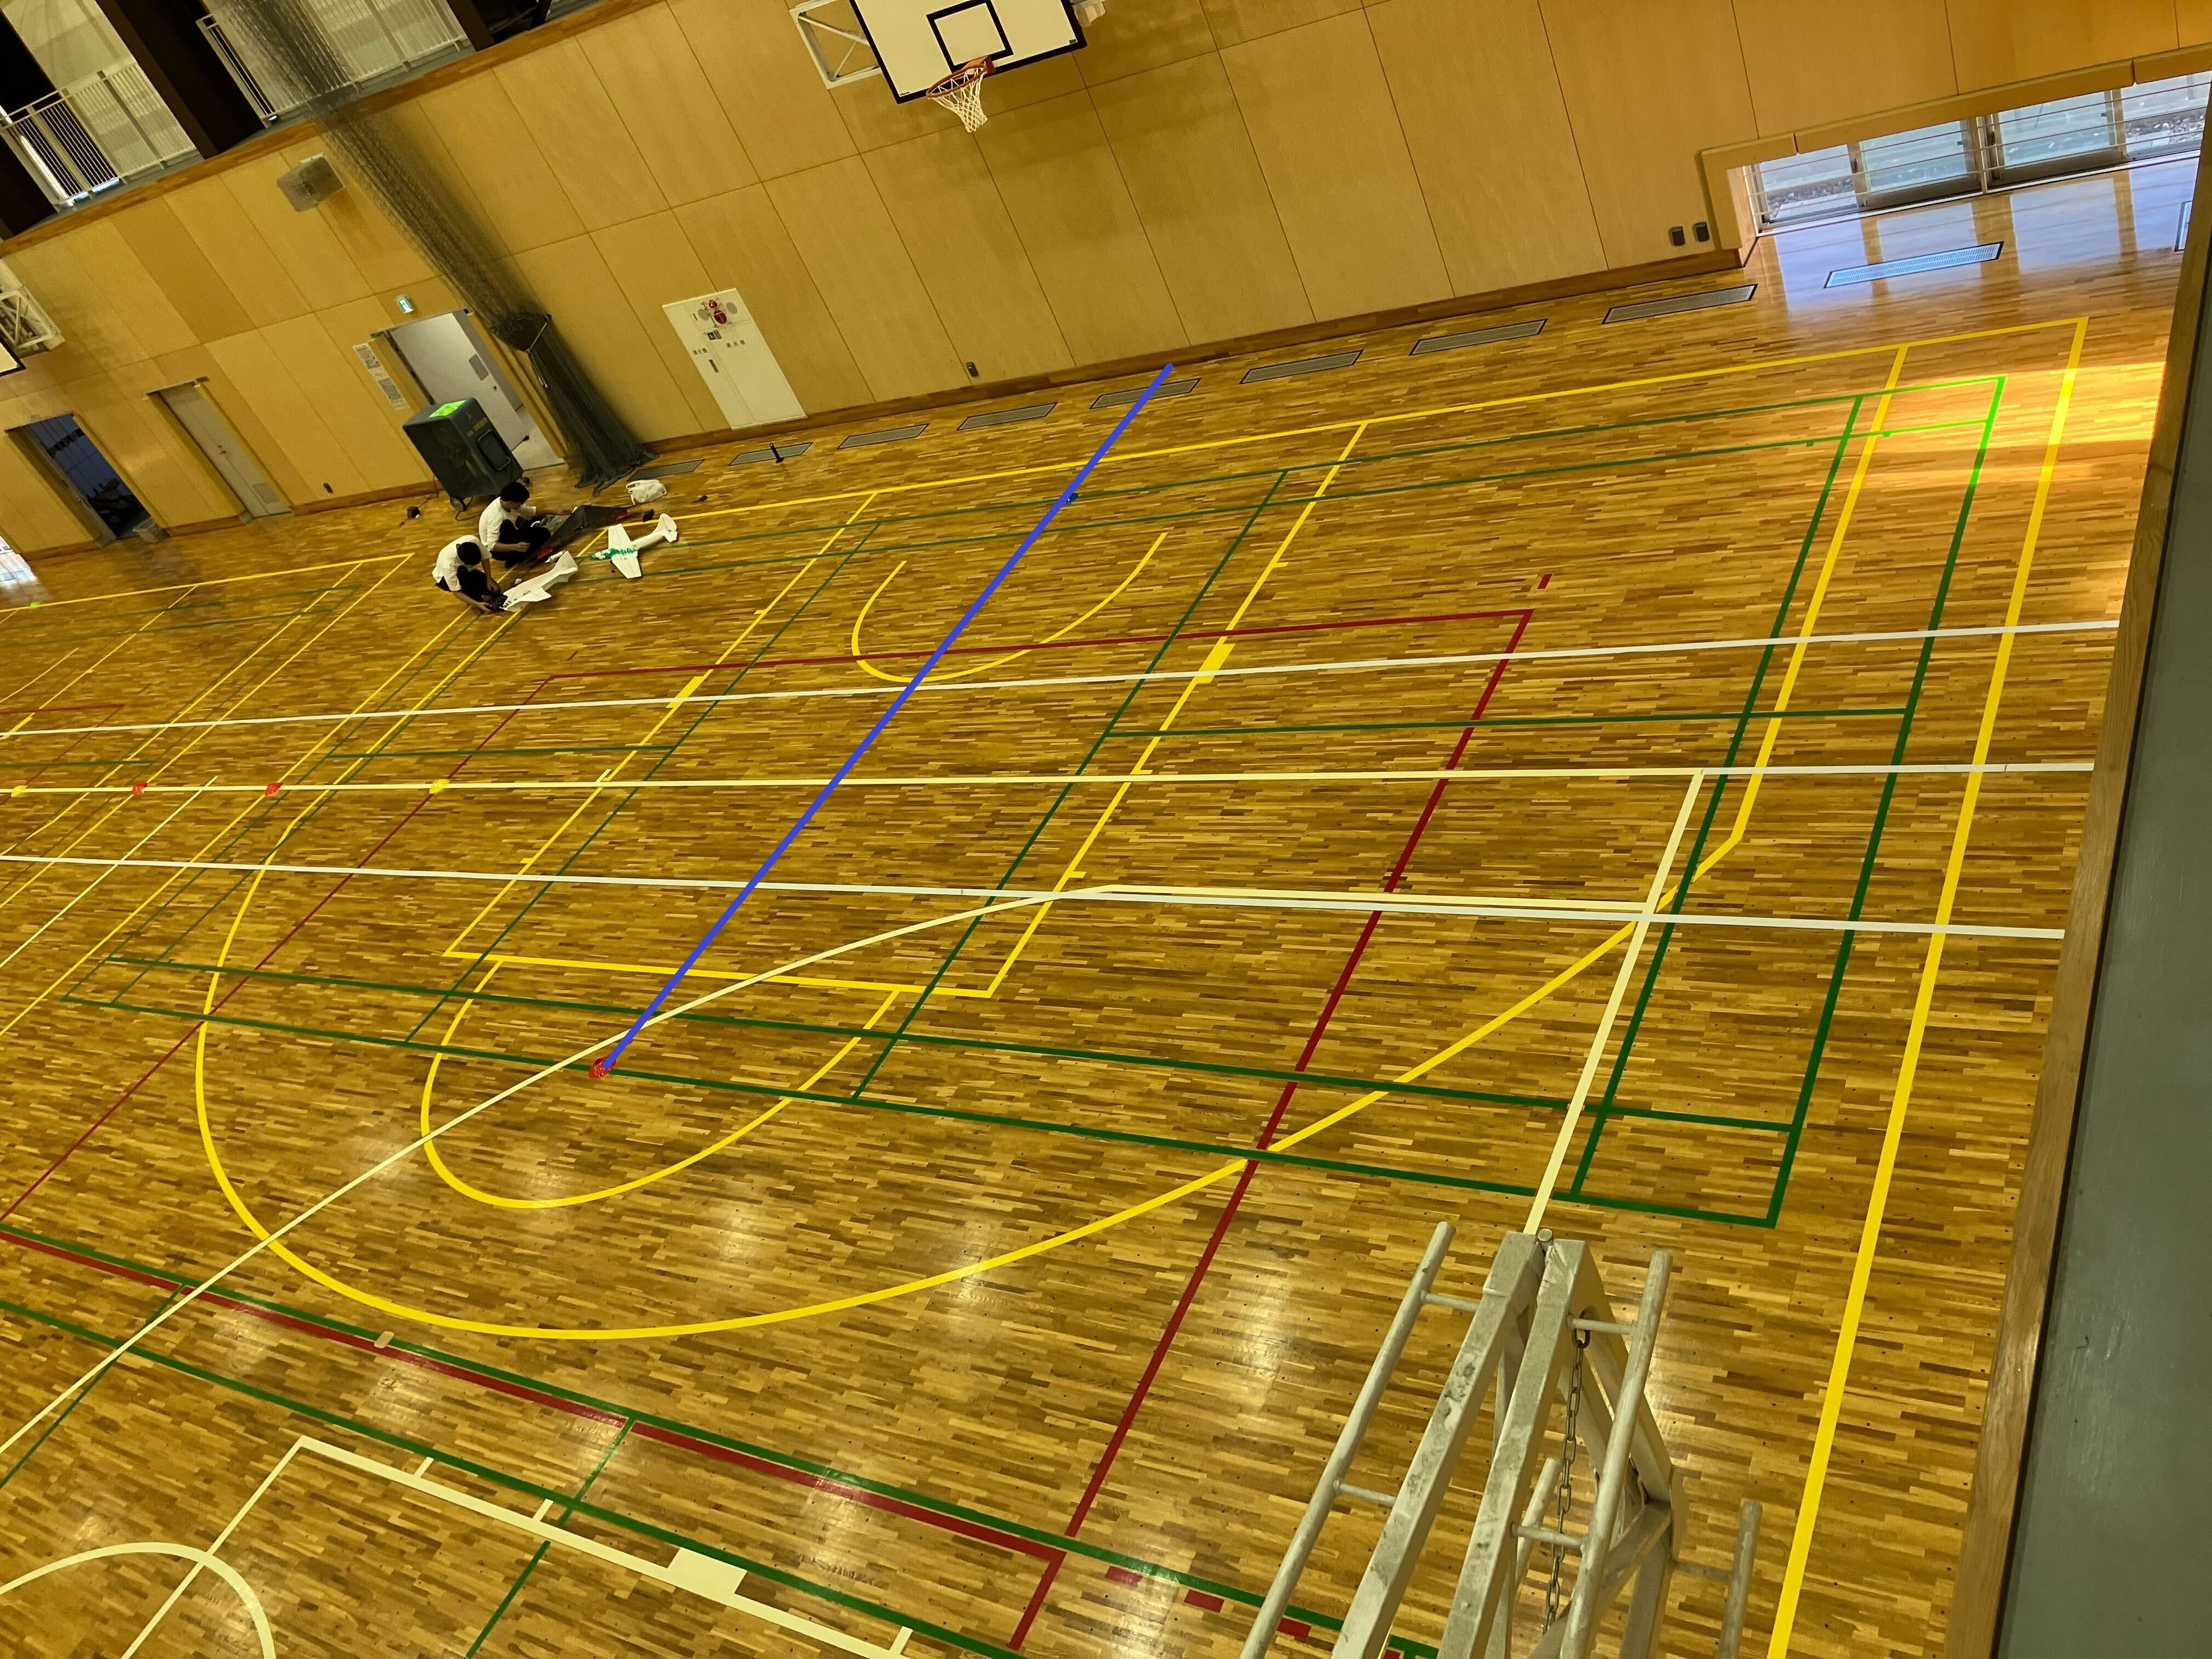
\includegraphics[width=70mm]{plane_poleTurn.jpg}
  \caption{ポール旋回}
  \label{fig::plane::poleTurn}
\end{figure}

\subsubsection{離着陸エリア}
図 \ref{fig::plane::landingZone} に離着陸エリアを示す.
\begin{itemize}
  \item オレンジの斜線部を滑走路とする
  \item 緑の斜線部と滑走路を合わせて離着陸エリアとする
  \item 体育館の壁面は離着陸エリア外とする
\end{itemize}
\begin{figure}[htb]
  \centering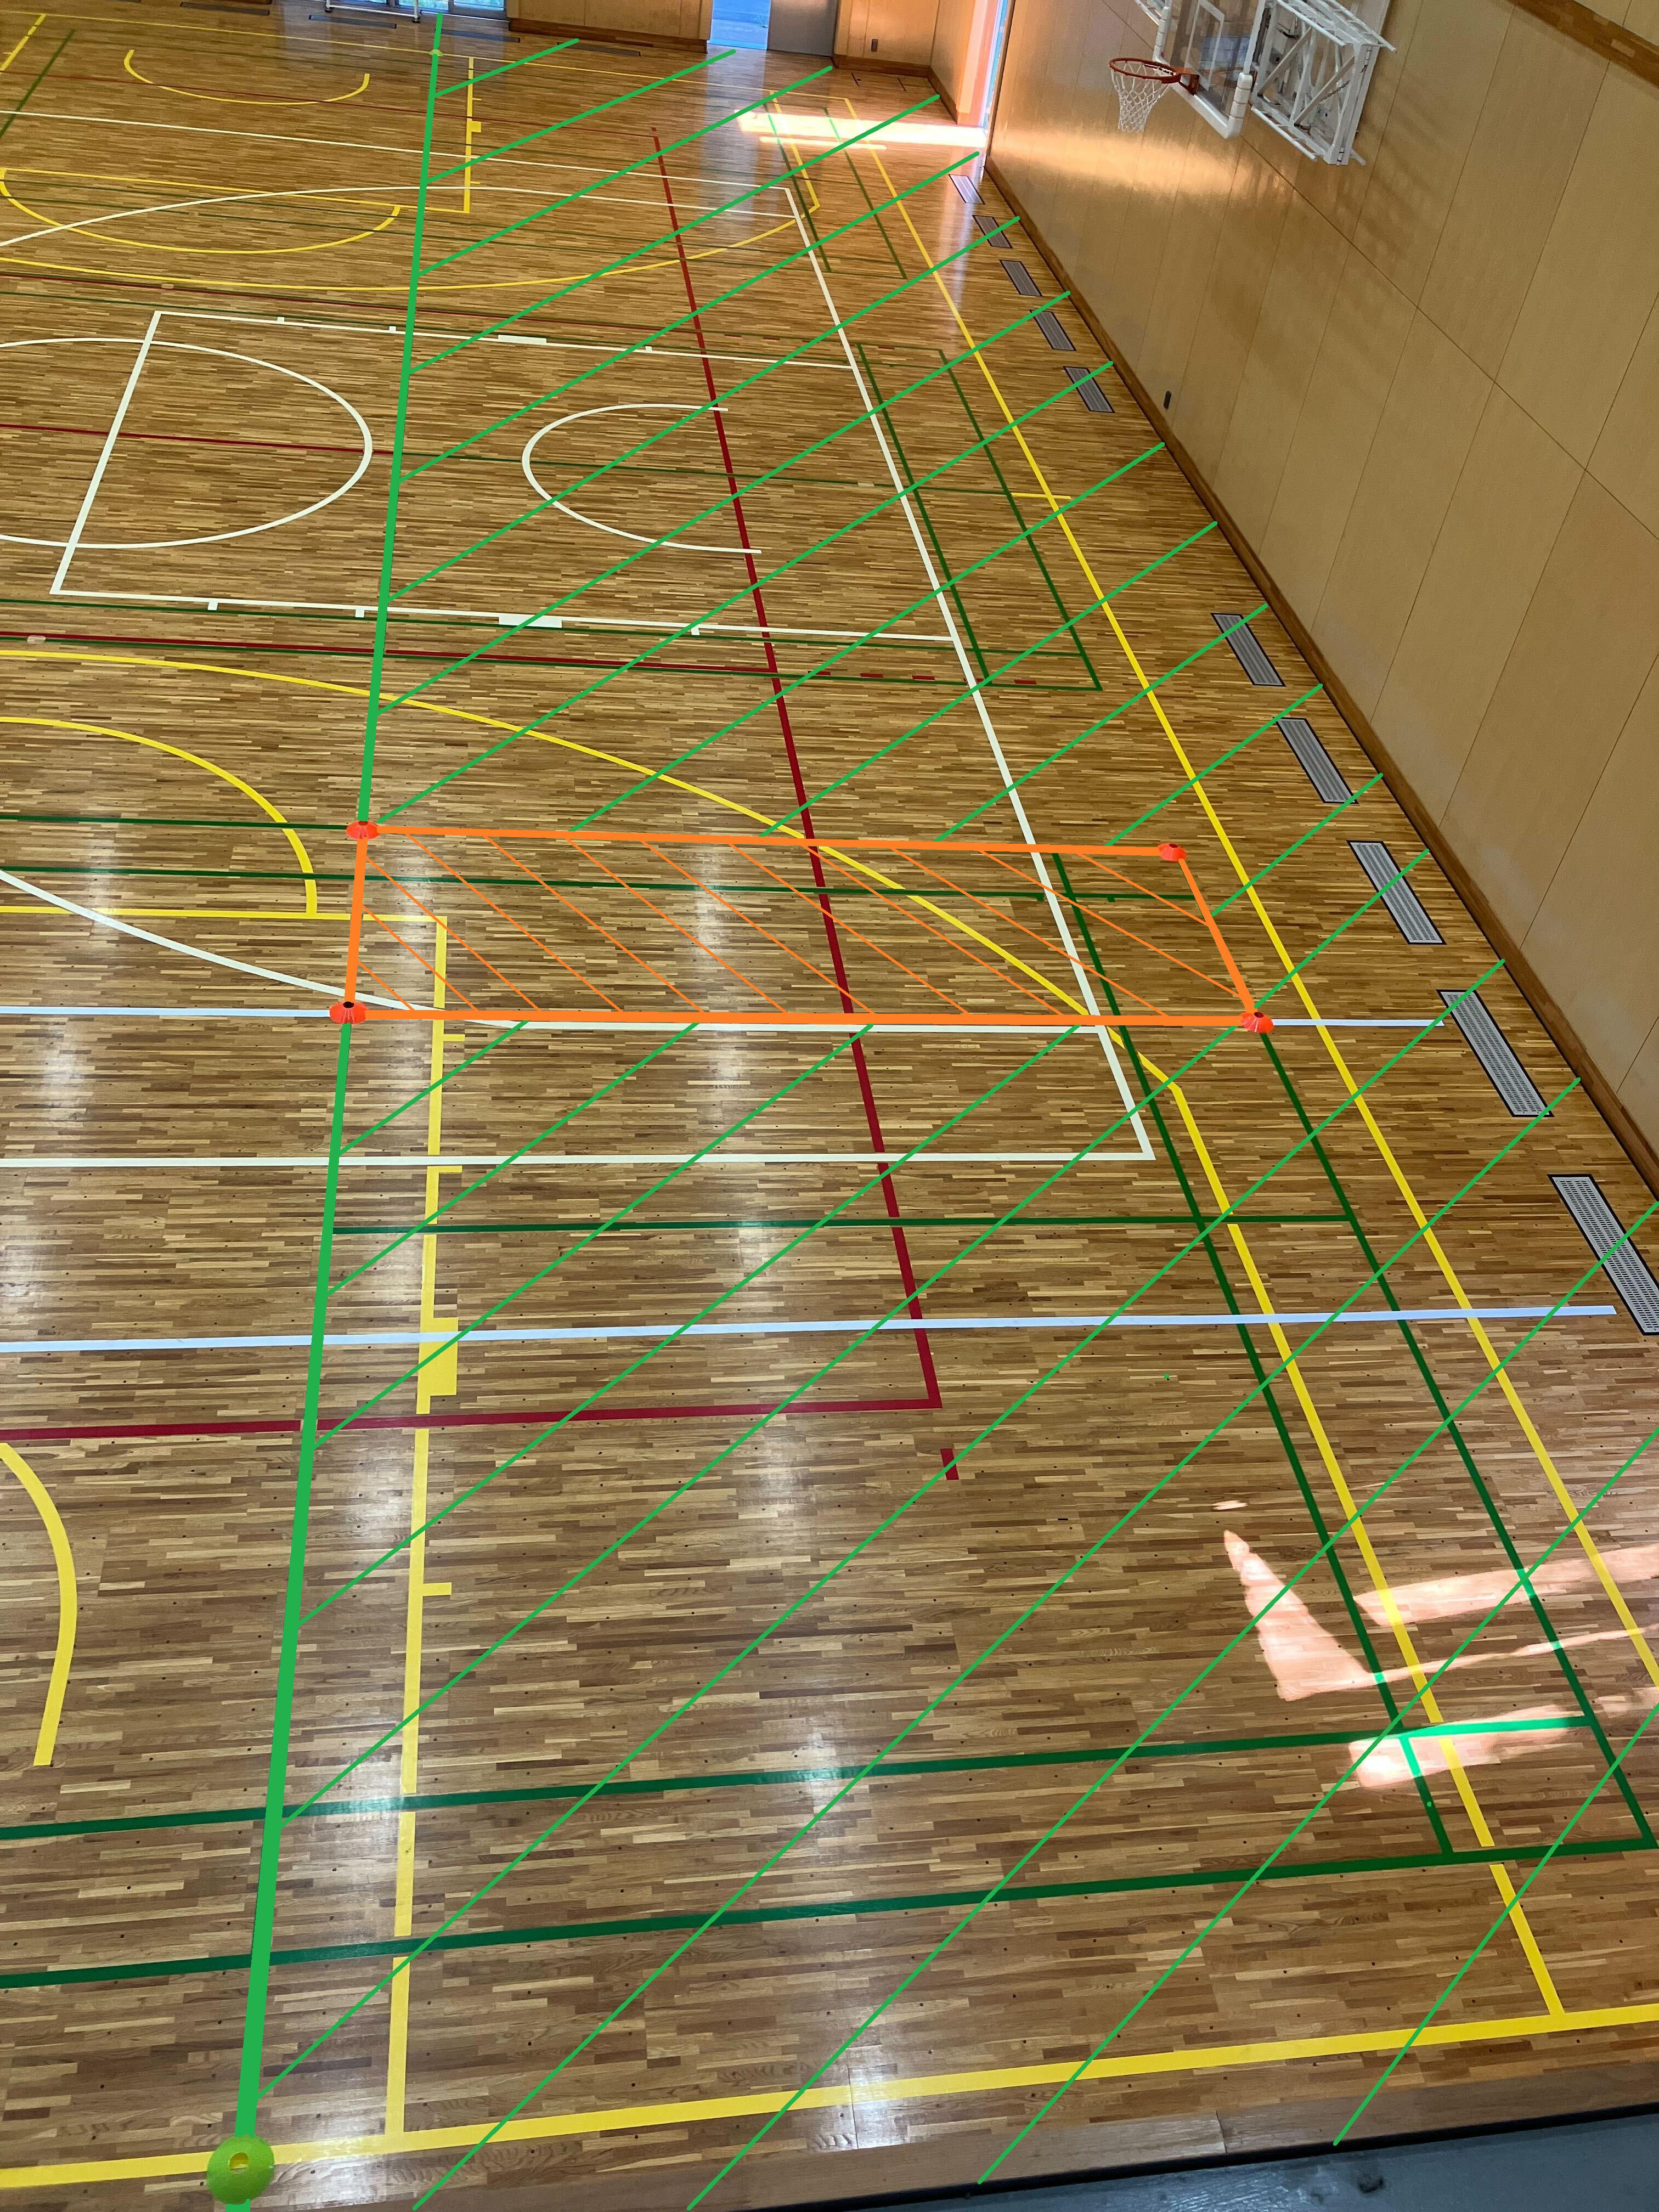
\includegraphics[width = 50mm,angle=90]{./plane_landingZone.jpg}
  \caption{離着陸エリア}
  \label{fig::plane::landingZone}
\end{figure}
\newpage